\documentclass{article}

\usepackage[most]{tcolorbox}
\usepackage{physics}
\usepackage{graphicx}
\usepackage{float}
\usepackage{amsmath}
\usepackage{amssymb}

\usepackage{tikz}

\usepackage[utf8]{inputenc}
\usepackage[a4paper, margin=1in]{geometry} % Controla los márgenes
\usepackage{titling}

\title{Mecánica Estadística }
\author{Manuel Garcia.}
\date{\today}

\renewcommand{\maketitlehooka}{%
  \centering
  \vspace*{0.05cm} % Espacio vertical antes del título
}

\renewcommand{\maketitlehookd}{%
  \vspace*{2cm} % Espacio vertical después de la fecha
}

\newcommand{\caja}[3]{%
  \begin{tcolorbox}[colback=#1!5!white,colframe=#1!25!black,title=#2]
    #3
  \end{tcolorbox}%
}

\begin{document}
\maketitle

\section{Indistinguibilidad en el Ensamble Canónico }
\subsection{Formulación cuántica de un sistema de $ N  $ partículas idénticas e indistinguibles no interactuantes entre sí y sin grado de libertad interno  }
$ N  $ partículas de masa $ m  $ idénticas e indistinguibles, no interactuantes entre sí y sin grado de libertad interno (como el spin). 
\begin{gather*}
  \hat H ^ {(N) } (\hat p_1, \cdots , \hat p_n ; \hat r _1 , \cdots , \hat r_N ) = \displaystyle\sum_{k = 1 }^{ N } \frac{\hat p_k ^2 }{2m } + \hat V (\hat r_1, \cdots , \hat r_N ) 
\end{gather*}

Ecuación de valores propios 
\begin{gather*}
  \left[- \frac{\hbar ^2 }{2m } \displaystyle\sum_{k= 1 }^{N }\nabla^2 _{\vec r_k } + \hat V (\vec r_1 , \cdots , \vec r_N ) \right] \Phi ^ {S|A } _{i_1,\cdots, i_N } (\vec r_1 , \cdots, \vec r _N ) = E _{i_1,\cdots , i_N } \Phi ^ {S|A } _{i_1,\cdots, i_N } (\vec r_1 , \cdots, \vec r _N )
\end{gather*}
La solución formal permite funciones de onda de posición simétrica o anti sinterizadas.

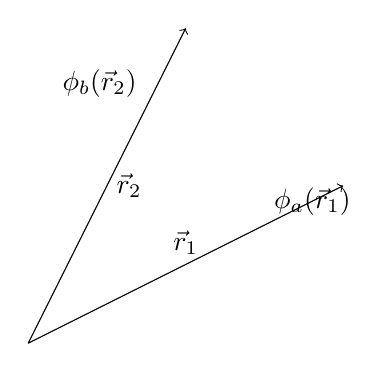
\begin{tikzpicture}
    % Dibuja el primer vector r1
    \draw[->] (0,0) -- (4,2) node[midway, above] {$\vec{r}_1$} node[near end, above right] {$\phi_a(\vec{r}_1)$};
    
    % Dibuja el segundo vector r2
    \draw[->] (0,0) -- (2,4) node[midway, right] {$\vec{r}_2$} node[near end, above left] {$\phi_b(\vec{r}_2)$};
\end{tikzpicture}
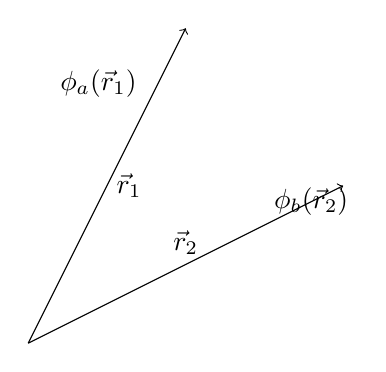
\begin{tikzpicture}
    % Dibuja el primer vector r1
    \draw[->] (0,0) -- (4,2) node[midway, above] {$\vec{r}_2$} node[near end, above right] {$\phi_b(\vec{r}_2)$};
    
    % Dibuja el segundo vector r2
    \draw[->] (0,0) -- (2,4) node[midway, right] {$\vec{r}_1$} node[near end, above left] {$\phi_a(\vec{r}_1)$};
\end{tikzpicture}

Estos dos estados son indistinguibles. 

Se puede construir una función de onda sinterizada y otra antisimetrizada.  
\begin{gather*}
  \Phi_{ab } ^ {(S )} (\vec r_1 , \vec r_2 ) \\
  \Phi_{ab } ^ {(A )} (\vec r_1 , \vec r_2 ) 
\end{gather*}

\hfill 

\hfill 

El Hamiltoniano para sistema de dos partículas 
\begin{gather*}
  \hat H ^ {(2) }= \frac{\hat p_1 ^2}{2m } + \frac{\hat p_2^2 }{2m } + V(\hat r_1 , \hat r_2 )
\end{gather*}
Adoptando la notación $ \hat H ^ {(2) }(\vec p_1, \vec p_2 , \vec r_1 , \vec r_1 ) = \hat H ^ {(2) }(i,j) $, y dado que $  V(\hat r_1 , \hat r_2 ) =  V(\hat r_2 , \hat r_1 ) $
\begin{gather*}
   \hat H ^ {(2) }(1,2) = \hat H ^ {(2) }(2,1)
\end{gather*}
A partir de la ecuación de valores propios tenemos: 
\begin{gather*}
   \hat H ^ {(2) }(2,1) \Phi ^ {S|A }(\vec r_1,\vec r_2 ) = E _{ab } \Phi _{ab } ^ {A|B } (\vec r_1 , \vec r_2 ) \\
   \hat H ^ {(2) }(1,2) \Phi ^ {S|A }(\vec r_2,\vec r_1 ) = E _{ab } \Phi _{ab } ^ {A|B } (\vec r_2 , \vec r_1 ) 
\end{gather*}

\hfill 

\hfill 

Introducimos el operador intercambio $ \hat P _{12 }  $ de la posición de la partícula 1 por la posición de la partícula 2, definido como: 
\begin{gather*}
  \hat P _{12 }  \Phi _{ab } ^ {S|A } (\vec r_1, \vec r_2 ) = \xi \Phi _{ab } ^ {S|A } (\vec r_2, \vec r_1 )
\end{gather*}
Donde $ \xi = 1  $ para la función de onda sinterizada $ (S) $ y $ \xi = - 1  $ para la función de onda antisimetrizada $ (A)  $.

$ \hat P _{12 }  $ tiene la propiedad de que a partir de dos intercambios sucesivos $ 1 \rightarrow 2  $ y $ 2 \rightarrow 1  $, se tiene la configuración original 
\begin{gather*}
  (\hat P _{12 } )^2 = 1  
\end{gather*}
Los valores propios pueden ser $ p = + 1  $ para la simetrizada y $ p = - 1  $ para la antisimetrizada 

Para la simetrizada:
\begin{gather}
  \vec P _{12 } \Phi _{ab } (\vec r_1, \vec r_2 ) = \vec P _{12 } \phi _a (\vec r_1) \phi_b(\vec r_2 ) = \phi_a (\vec r_2 ) \phi_b (\vec r_1 )
\end{gather}

Para la antisimetrizada: 
\begin{gather*}
  \vec P _{12 } \Phi _{ab } (\vec r_1, \vec r_2 ) = \vec P _{12 } \phi _a (\vec r_1) \phi_b(\vec r_2 ) = - \phi_a (\vec r_2 ) \phi_b (\vec r_1 )
\end{gather*}

\hfill 

\hfill 

Tenemos que: 
\begin{gather*}
  \Phi _{ab }  ^ {(S|A)} (\vec r_1, \vec r_2 ) = C_2 ^ {(S|A)} [\phi _{a }(\vec r_1)\phi _{b }(\vec r_2) + \xi \phi _{a }(\vec r_2)\phi _{a }(\vec r_1) ]  \\
  1 = \bra{\Phi _{ab }  ^ {(S|A)}}\ket{\Phi _{ba }  ^ {(S|A)}} 
\end{gather*}
Resolviendo para hallar $ C_2 ^ {(S|A )} $
\begin{gather*}
   C_2 ^ {(S|A )} = \frac{1}{\sqrt{2 } }
\end{gather*}

Entonces tenemos que 
\begin{gather*}
  \Phi _{ab }  ^ {(S|A)} (\vec r_1, \vec r_2 ) = \frac{1}{\sqrt{2} } [\phi _{a }(\vec r_1)\phi _{b }(\vec r_2) + \xi \phi _{a }(\vec r_2)\phi _{a }(\vec r_1) ] 
\end{gather*}

Se definen los operadores simetrización $ \hat S _{12 }  $ y antisimetrización  
\begin{gather*}
   \hat S _{12 } = \frac{1}{\sqrt{2 } } (\hat e + \hat P _{12 } )\\
  \hat A _{12 } = \frac{1}{\sqrt{2 } } (\hat e - \hat P _{12 } )
\end{gather*}
Donde $ \hat e  $ representa el operador identidad y $ \hat P  $ el operador intercambio de la posición de la partícula 1 y 2 
\begin{gather*}
   \Phi _{ab }  ^ {(S)} (\vec r_1, \vec r_2 ) = \hat S _{12 } \Phi _{ab }  (\vec r_1, \vec r_2 ) = \frac{1}{\sqrt{2} } [\Phi _{a }(\vec r_1)\Phi _{b }(\vec r_2) + \xi \Phi _{a }(\vec r_2)\Phi _{a }(\vec r_1) ] \\
   \Phi _{ab }  ^ {(A)} (\vec r_1, \vec r_2 ) = \hat A _{12 } \Phi _{ab }  (\vec r_1, \vec r_2 ) = \frac{1}{\sqrt{2} } [\Phi _{a }(\vec r_1)\Phi _{b }(\vec r_2) - \xi \Phi _{a }(\vec r_2)\Phi _{a }(\vec r_1) ] 
\end{gather*}

\hfill 

\hfill 

\textbf{Forma alternativa } Para el caso de la función de onda simetrizada, se usa el permanente (determinante de Slater con todos los términos de la suma positivos). Para el caso de la función de onda antisimetrizada se usa el determinante de Slater usual.

Las dos partículas se pueden encontrar en cualquiera de los 2 estados de partícula simple 
\begin{gather*}
  \ket{\phi _{i_1 } } \rightarrow \epsilon _{i_1 } \\
  \ket{\phi _{i_2 } } \rightarrow \epsilon _{i_2 }  \\
\end{gather*}

Obtenemos: 
\begin{gather*}
  \Phi _{i_1, i_2 } (\vec r_1, \vec r_2 ) = \phi _{i_1 } (\vec r_1 )\phi _{i_2 } (\vec r_2 ) \\
  \hat P _{12 } \Phi _{i_1, i_2 } (\vec r_1, \vec r_2 ) = \phi _{i_1 } (\vec r_2 )\phi _{i_2 } (\vec r_1 ) 
\end{gather*}

En esta notación: 
\begin{gather*}
  \Phi ^ {(S|A ) } _{i_2 , i _1 } (\vec r _ 1, \vec r_2 ) = \psi ^ {\pm } _{i_1,i_2 } (\vec r_1, \vec r_2 ) = \frac{1}{\sqrt{2 } } 
  \begin{vmatrix}
      \phi _{i_1 } (\vec r_1 ) & \phi _{i_1 } (\vec r_2 ) \\
      \phi _{i_2 } (\vec r_1 ) & \phi _{i_2 } (\vec r_2 )
  \end{vmatrix}  
\end{gather*}

\subsection{Sistema de tres partículas idénticas, indistinguibles e independientes } 
Tres partículas idénticas, indistinguibles e independientes: 
\begin{gather*}
  \hat H ^ {(3)} (\vec p_1, \vec p_2,\vec p_3,\vec p_1,\vec p_2,\vec p_3) = \frac{\hat p_1^2 }{2m } + \frac{\hat p_2^2 }{2m } + \frac{\hat p_3^2 }{2m } + V(\hat r_1, \hat r_2 , \hat r_3 )
\end{gather*}
Nivel de energía asociado: 
\begin{gather*}
  E _{abc } = \epsilon_a + \epsilon_b + \epsilon_c  
\end{gather*}
Con el mismo proceso que se realizo para dos partículas obtenemos: 
\begin{gather*}
  C_3 ^ {(A|B )} = \frac{1}{\sqrt{3! } } = \frac{1}{\sqrt{6 } } \\
  \hat S _{123 } = \frac{1}{\sqrt{3! } } (\hat e + \hat P _{12 }  + \hat P _{213 } + \hat P _{13 } + \hat P _{123 } + \hat P _{23 }) \\
  \hat A _{123 } = \frac{1}{\sqrt{3! } } (\hat e - \hat P _{12 }  + \hat P _{213 } - \hat P _{13 } + \hat P _{123 } - \hat P _{23 }) 
\end{gather*}

\hfill 

\hfill 

\begin{gather*}
  \Phi ^ {(S|A ) } _{i_1 , i _2, i_3 } (\vec r _ 1, \vec r_2, \vec r_3 ) = \psi ^ {\pm } _{i_1,i_2, i_3 } (\vec r_1, \vec r_2 , \vec r_3) = \frac{1}{\sqrt{3! } } 
  \begin{vmatrix}
      \phi _{i_1 } (\vec r_1 ) & \phi _{i_1 } (\vec r_2 ) & \phi _{i_1 } (\vec r_3 )  \\
      \phi _{i_2 } (\vec r_1 ) & \phi _{i_2 } (\vec r_2 ) & \phi _{i_2 } (\vec r_3 )  \\
      \phi _{i_3 } (\vec r_1 ) & \phi _{i_3 } (\vec r_2 ) & \phi _{i_3 } (\vec r_3 ) 
  \end{vmatrix}  
\end{gather*}

\hfill 

\hfill 

\hfill 

\textbf{Para $ N  $ partículas}: 
\begin{gather*}
  \Phi _{i_1,\cdots, i_N)(\vec r_1, \cdots, \vec r_N )} = \phi _{i_1 } (\vec r_1 ) \phi _{i_2 } (\vec r_2 )\phi _{i_N } \cdots (\vec r_N ) \\
  E _{i_1, \cdots, i_N } = \epsilon _{i_1 }  + \epsilon _{i_2 } + \cdots + \epsilon _{i_N } \\
  \Phi ^ {(S|A ) } _{i_1 , \cdots, i_N } (\vec r _ 1, \cdots, \vec r_N ) = \psi ^ {\pm } _{i_1,\cdots, i_N } (\vec r_1,\cdots , \vec r_N) = \frac{1}{\sqrt{N! } } 
  \begin{vmatrix}
      \phi _{i_1 } (\vec r_1 ) & \cdots & \phi _{i_1 } (\vec r_N )  \\
      \vdots & \ddots & \vdots  \\
      \phi _{i_N } (\vec r_1 ) & \cdots & \phi _{i_N } (\vec r_N ) 
  \end{vmatrix}  
\end{gather*}


\end{document}
